\documentclass[12pt, fleqn]{article}

\usepackage[left=0.75in, right=0.75in, bottom=0.75in, top=1.0in]{geometry}
\usepackage{amsmath}
\usepackage{amssymb}
\usepackage{amsthm}
\usepackage{mathtools}
\usepackage{hyperref}
\usepackage{ulem}
\usepackage{enumitem}
\usepackage{floatrow}
\usepackage{graphicx}
\usepackage{subcaption}
\usepackage[export]{adjustbox}
\usepackage{sectsty}
\usepackage{enumitem}
\renewcommand{\thesubsubsection}{(\roman{subsubsection})}

\usepackage[dvipsnames]{xcolor}
\usepackage[perpage]{footmisc}

\usepackage{fancyhdr}
\pagestyle{fancy}
\fancyhf{}
\lhead{190100044}
\rhead{Assignment 4}
\renewcommand{\footrulewidth}{1.0pt}
\cfoot{Page \thepage}

\setlength{\parindent}{0em}

\title{Assignment 4}
\author{Devansh Jain, 190100044}
\date{30th Oct 2021}

\DeclareMathOperator*{\argmax}{arg\,max}
\DeclareMathOperator*{\argmin}{arg\,min}

\begin{document}

% \pagenumbering{gobble}
\maketitle
\tableofcontents
\thispagestyle{empty}
\setcounter{page}{0}

\newpage
\section{Clustering}
\subsection{CS 335 KMeans Implementation}
\subsubsection{}
Code for the class \verb!Kmeans! updated in notebook.

\subsubsection{}
For Dataset 1, we observe that the algorithm works well as the dataset is linearly separable. \\
For Dataset 2, we get algorithm converges to same centroids (except flipping of color) but these are not able to separate the clusters as the dataset isn't linearly separable. \\
For Dataset 2, we get different centroids for different initialization. This can be explained by the radial symmetry. \\

\begin{figure}[H]
    \centering
    \begin{subfigure}[H]{0.35\textwidth}
        \centering
        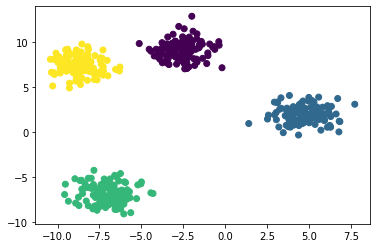
\includegraphics[width=\textwidth]{plots/D1/orig.png}
        \caption[]{True clusters}
    \end{subfigure}
    \begin{subfigure}[H]{0.35\textwidth}
        \centering
        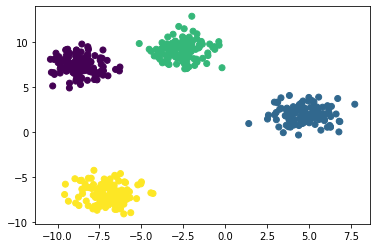
\includegraphics[width=\textwidth]{plots/D1/0.png}
        \caption[]{Seed = 0}
    \end{subfigure}
    \vskip\baselineskip
    \begin{subfigure}[H]{0.35\textwidth}
        \centering
        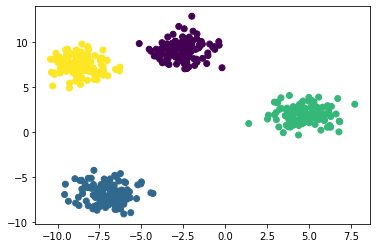
\includegraphics[width=\textwidth]{plots/D1/11.png}
        \caption[]{Seed = 11}
    \end{subfigure}
    \begin{subfigure}[H]{0.35\textwidth}
        \centering
        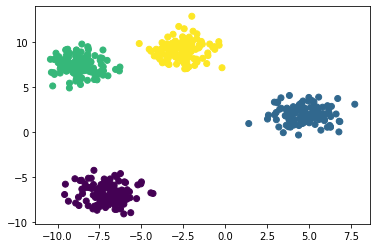
\includegraphics[width=\textwidth]{plots/D1/123.png}
        \caption[]{Seed = 123}
    \end{subfigure}
    \caption[]{Dataset 1}
\end{figure}

\begin{figure}[H]
    \centering
    \begin{subfigure}[H]{0.35\textwidth}
        \centering
        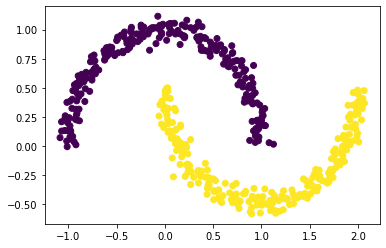
\includegraphics[width=\textwidth]{plots/D2/orig.png}
        \caption[]{True clusters}
    \end{subfigure}
    \begin{subfigure}[H]{0.35\textwidth}
        \centering
        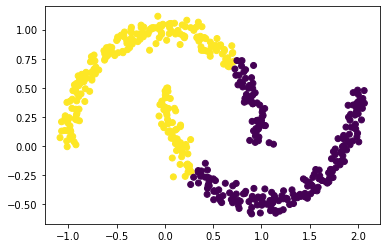
\includegraphics[width=\textwidth]{plots/D2/0.png}
        \caption[]{Seed = 0}
    \end{subfigure}
    \vskip\baselineskip
    \begin{subfigure}[H]{0.35\textwidth}
        \centering
        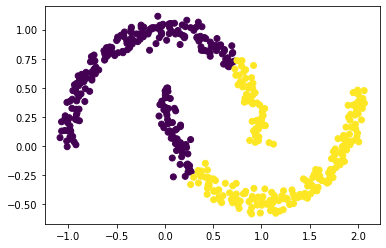
\includegraphics[width=\textwidth]{plots/D2/11.png}
        \caption[]{Seed = 11}
    \end{subfigure}
    \begin{subfigure}[H]{0.35\textwidth}
        \centering
        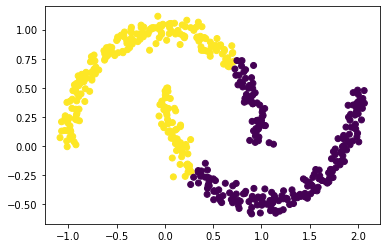
\includegraphics[width=\textwidth]{plots/D2/123.png}
        \caption[]{Seed = 123}
    \end{subfigure}
    \caption[]{Dataset 2}
\end{figure}

\begin{figure}[H]
    \centering
    \begin{subfigure}[H]{0.35\textwidth}
        \centering
        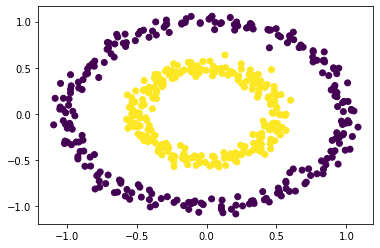
\includegraphics[width=\textwidth]{plots/D3/orig.png}
        \caption[]{True clusters}
    \end{subfigure}
    \begin{subfigure}[H]{0.35\textwidth}
        \centering
        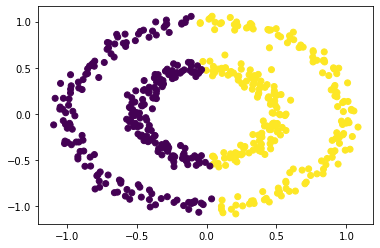
\includegraphics[width=\textwidth]{plots/D3/0.png}
        \caption[]{Seed = 0}
    \end{subfigure}
    \vskip\baselineskip
    \begin{subfigure}[H]{0.35\textwidth}
        \centering
        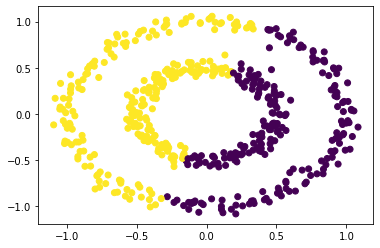
\includegraphics[width=\textwidth]{plots/D3/11.png}
        \caption[]{Seed = 11}
    \end{subfigure}
    \begin{subfigure}[H]{0.35\textwidth}
        \centering
        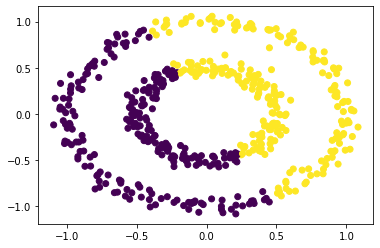
\includegraphics[width=\textwidth]{plots/D3/123.png}
        \caption[]{Seed = 123}
    \end{subfigure}
    \caption[]{Dataset 3}
\end{figure}

\subsubsection{}
We need to initialize the centroids at different locations. \\
One of the fastest method is to randomly choose \verb!n_clusters! data points. This method is also known as Forgy Initialization. \\
I have implemented the algorithm with this initialization. \\
This initialization method makes sense because the clusters detected through KMeans are more probable to be near the modes present in data. \\
By randomly choosing points from data, we are making it more probable to get a point that lies close to the modes.


\newpage
\section{Kernel design and Kernelized clustering}
\subsection{CS 337: Proving Kernel Validity}
We are going to use the following property of kernels from Lecture slides (Lecture 11):
\begin{equation*}
    \begin{aligned}
        K(x,y) = \sum_{d=1}^r \alpha_d(x^T y)^d \text{ where } \alpha_d \ge 0 \text{ is a kernel } (r \text{ can be } \infty)
    \end{aligned}
\end{equation*}

Another property of kernels which we are going to use is:
\begin{equation*}
    \begin{aligned}
         & K(x, y) \text{ is a kernel } \implies K'(x, y) = f(x) f(y) K(x, y) \text{ is also a kernel} \\
         & \text{Corresponding feature map, } \phi'(x) := f(x) \phi(x)
    \end{aligned}
\end{equation*}


An important property of exponential function which we are going to exploit is:
\begin{equation*}
    \begin{aligned}
        \exp(x) = \sum_{k=0}^{\infty} \frac{x^k}{k!}
    \end{aligned}
\end{equation*}

Using the above properties, we can conclude that $\exp(\alpha x^T y)$ where $\alpha \ge 0$ is a kernel.

Now, if take $\alpha = \dfrac{1}{\sigma^2}$ and $f(x) = \exp\bigg(- \dfrac{x^T x}{2 \sigma^2}\bigg)$, we get: \\
$K_\alpha (x, y) = \exp\bigg(- \dfrac{||x - y||^2}{2 \sigma^2}\bigg) = \exp\bigg(- \dfrac{x^T x}{2 \sigma^2}\bigg) \exp\bigg(- \dfrac{y^T y}{2 \sigma^2}\bigg) \exp\bigg(\dfrac{x^T y}{\sigma^2}\bigg)$ is a kernel.

Hence, proved. \hfill $\qed$


\subsection{CS 337: Simple Kernel Design}
\subsubsection{}
We proved in Lecture slides (Lecture 13, Part 2) that the vanilla KMeans algorithm would converge in finite number of iterations (say, $N$). \\
Without loss of generality, let $r_1 \ge r_2$. \\
For the sake of contradiction, let's assume that after $N$ iterations we get ${\mu_1, \mu_2}$ which can correctly classify the clusters. Obviously, $\mu_1 \neq \mu_2$. \\
So, blue points have $Pr_1 = 1$ and $Pr_2 = 0$ while red points have $Pr_1 = 0$ and $Pr_2 = 1$. \\
As the algorithm has converged, the $Pr$s for all points and $\mu$s won't change any further. \\

The decision boundary would be $f(x) = \bigg(x - \dfrac{\mu_1 + \mu_2}{2}\bigg) \cdot (\mu_2 - \mu_1) = (x \cdot (\mu_2 - \mu_1)) - \dfrac{||\mu_1 - \mu_2||^2}{2}$. \\
This decision boundary is linear in $x$, therefore, due to radial symmetry some of blue and red points would be on same side. \\
However, we know that $Pr_1 = 0$ for red points and $Pr_1 = 1$ for blue points. So in $(N+1)^{th}$ iteration, the values of $Pr$s would change for some points. \\

This leads to contradiction. \\
Thus, even after convergence, the vanilla KMeans algorithms won't be able to correctly classify the clusters for any value of $r_1$ and $r_2$.

\subsubsection{}
We see that the two clusters differ in distance from origin. \\
We propose $\phi(x) = ||x||_2$. Thus, $K(x, x') = ||x||_2 ||x'||_2$. \\
$\int_x \int_{x'} K(x, x') g(x) g(x') dx dx' = \bigg( \int_x ||x||_2 g(x) dx \bigg) \bigg( \int_{x'} ||x'||_2 g(x') dx' \bigg) = \bigg( \int_x ||x||_2 g(x) dx \bigg)^2 \ge 0$ \\
Therefore, chosen kernel function is a valid kernel.

\bigskip
\bigskip

Code for the class \verb!Kmeans_Kernel! updated in notebook. \\

For Dataset 3, we observe that the algorithm works well as the dataset is linearly separable in the above defined $\phi$-space. \\
For Dataset 3 shifted by $(5, 5)$, we observe that the algorithm works well after zero-centering the data. \\

\begin{figure}[H]
    \centering
    \begin{subfigure}[H]{0.35\textwidth}
        \centering
        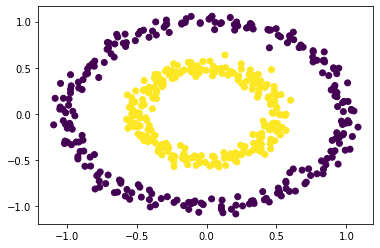
\includegraphics[width=\textwidth]{plots/D3/orig.png}
        \caption[]{True clusters}
    \end{subfigure}
    \begin{subfigure}[H]{0.35\textwidth}
        \centering
        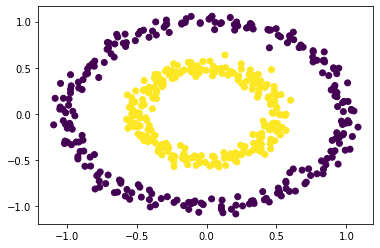
\includegraphics[width=\textwidth]{plots/D3/K0.png}
        \caption[]{Seed = 0}
    \end{subfigure}
    \vskip\baselineskip
    \begin{subfigure}[H]{0.35\textwidth}
        \centering
        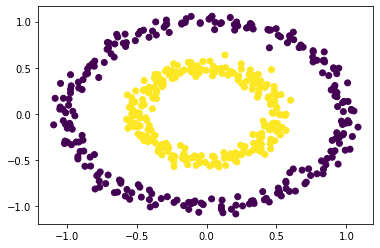
\includegraphics[width=\textwidth]{plots/D3/K11.png}
        \caption[]{Seed = 11}
    \end{subfigure}
    \begin{subfigure}[H]{0.35\textwidth}
        \centering
        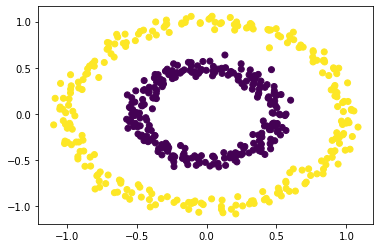
\includegraphics[width=\textwidth]{plots/D3/K123.png}
        \caption[]{Seed = 123}
    \end{subfigure}
    \caption[]{Dataset 3}
\end{figure}

\begin{figure}[H]
    \centering
    \begin{subfigure}[H]{0.35\textwidth}
        \centering
        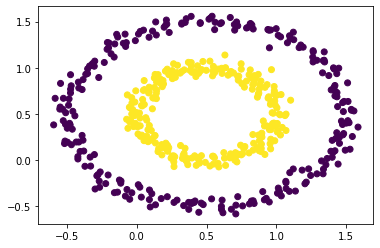
\includegraphics[width=\textwidth]{plots/D3_shifted/orig.png}
        \caption[]{True clusters}
    \end{subfigure}
    \begin{subfigure}[H]{0.35\textwidth}
        \centering
        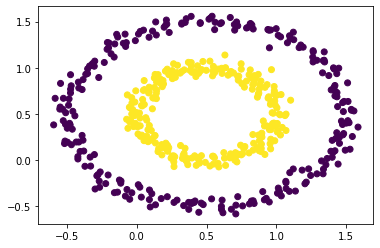
\includegraphics[width=\textwidth]{plots/D3_shifted/K0.png}
        \caption[]{Seed = 0}
    \end{subfigure}
    \vskip\baselineskip
    \begin{subfigure}[H]{0.35\textwidth}
        \centering
        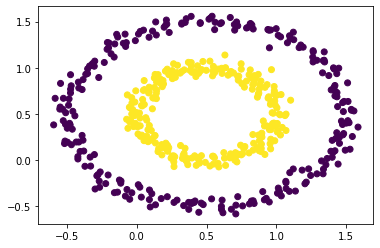
\includegraphics[width=\textwidth]{plots/D3_shifted/K11.png}
        \caption[]{Seed = 11}
    \end{subfigure}
    \begin{subfigure}[H]{0.35\textwidth}
        \centering
        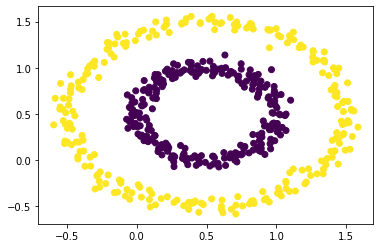
\includegraphics[width=\textwidth]{plots/D3_shifted/K123.png}
        \caption[]{Seed = 123}
    \end{subfigure}
    \caption[]{Dataset 3 shifted by $(5, 5)$}
\end{figure}



\end{document}
